%%%%%%%%%%%%%%%%%%%%%%%%%%%%%%%%%%%%%%%%%%%%%%%%%%%%%%%%%%%%
% 3.12 DISCRETE GEOMETRY
% The Composition of Advanced Mathematics
%%%%%%%%%%%%%%%%%%%%%%%%%%%%%%%%%%%%%%%%%%%%%%%%%%%%%%%%%%%%

\section{Discrete Geometry}
\label{sec:discrete-geometry}

\prerequisite{
Euclidean Geometry, Vector Geometry, Affine Geometry,
Convex Geometry, basic Linear Algebra, and elementary Combinatorics.
}

\learningobjectives{
By the end of this section, the reader should be able to:
\begin{itemize}
    \item explain the scope of discrete geometry;
    \item distinguish discrete geometric objects from continuous ones;
    \item work with finite point configurations;
    \item describe lattices and fundamental regions;
    \item define lattice points and lattice polytopes;
    \item compute areas of lattice polygons using Pick's theorem;
    \item explain the geometry of numbers at an introductory level;
    \item state Minkowski's convex body theorem;
    \item describe packings, coverings, and tilings;
    \item compute packing density in simple configurations;
    \item distinguish translational, lattice, and general packings;
    \item describe Voronoi diagrams and Delaunay triangulations;
    \item recognize triangulations of point sets and polygons;
    \item state Euler's polyhedron formula;
    \item explain basic polyhedral combinatorics;
    \item recognize regular and convex polytopes;
    \item describe geometric graphs and proximity structures;
    \item explain basic incidence problems;
    \item recognize the role of discrete geometry in coding,
    optimization, crystallography, and computational geometry.
\end{itemize}
}

%%%%%%%%%%%%%%%%%%%%%%%%%%%%%%%%%%%%%%%%%%%%%%%%%%%%%%%%%%%%
\subsection{What Is Discrete Geometry?}
\label{subsec:what-is-discrete-geometry}
%%%%%%%%%%%%%%%%%%%%%%%%%%%%%%%%%%%%%%%%%%%%%%%%%%%%%%%%%%%%

Discrete geometry studies geometric structures built from objects that are
finite, countable, combinatorial, or otherwise separated rather than
continuously distributed.

Typical objects include

\[
\boxed{
\text{finite point sets},
\quad
\text{lattices},
\quad
\text{polytopes},
\quad
\text{packings},
\quad
\text{tilings},
\quad
\text{geometric graphs}.
}
\]

The subject lies at the intersection of geometry and combinatorics.

\begin{conceptbox}
Continuous geometry asks about shapes, curves, surfaces, and spaces.

Discrete geometry often asks what can happen when geometric objects are
arranged in finite or countable configurations.
\end{conceptbox}

%%%%%%%%%%%%%%%%%%%%%%%%%%%%%%%%%%%%%%%%%%%%%%%%%%%%%%%%%%%%
\subsection{Discrete Point Sets}
\label{subsec:discrete-point-sets}
%%%%%%%%%%%%%%%%%%%%%%%%%%%%%%%%%%%%%%%%%%%%%%%%%%%%%%%%%%%%

A point set

\[
S\subseteq\R^n
\]

is called \emph{discrete} if its points are locally isolated.

Informally, each point can be surrounded by a sufficiently small
neighborhood containing no other points of \(S\).

Finite point sets are automatically discrete.

The integer lattice

\[
\Z^n
\]

is an important infinite discrete set.

%%%%%%%%%%%%%%%%%%%%%%%%%%%%%%%%%%%%%%%%%%%%%%%%%%%%%%%%%%%%
\subsection{Point Configurations}
\label{subsec:point-configurations}
%%%%%%%%%%%%%%%%%%%%%%%%%%%%%%%%%%%%%%%%%%%%%%%%%%%%%%%%%%%%

A finite collection

\[
\boxed{
P=\{p_1,\ldots,p_m\}\subseteq\R^n
}
\]

is called a \emph{point configuration}.

Questions about point configurations include:

\begin{itemize}
    \item Which points lie on a common line?
    \item Which points determine the convex hull?
    \item How many distances occur?
    \item How many triangles can be formed?
    \item Which points are nearest neighbors?
    \item Can the points be separated by a hyperplane?
    \item How can the configuration be triangulated?
\end{itemize}

%%%%%%%%%%%%%%%%%%%%%%%%%%%%%%%%%%%%%%%%%%%%%%%%%%%%%%%%%%%%
\subsection{General Position}
\label{subsec:discrete-general-position}
%%%%%%%%%%%%%%%%%%%%%%%%%%%%%%%%%%%%%%%%%%%%%%%%%%%%%%%%%%%%

Geometric problems often become simpler when degeneracies are excluded.

For example, a planar point configuration is often said to be in
\emph{general position} when no three points are collinear.

In \(\R^n\), a common general-position assumption is that no \(n+1\) points
lie in a common affine hyperplane, although the exact meaning depends on the
problem.

\begin{warningbox}
``General position'' does not have one universal definition.

Its meaning must be specified for the geometric problem being studied.
\end{warningbox}

%%%%%%%%%%%%%%%%%%%%%%%%%%%%%%%%%%%%%%%%%%%%%%%%%%%%%%%%%%%%
\subsection{Lattices}
\label{subsec:discrete-lattices}
%%%%%%%%%%%%%%%%%%%%%%%%%%%%%%%%%%%%%%%%%%%%%%%%%%%%%%%%%%%%

\begin{definitionbox}{Lattice}
A \emph{lattice} in \(\R^n\) is a set of the form

\[
\boxed{
\Lambda
=
\left\{
m_1v_1+\cdots+m_nv_n:
m_i\in\Z
\right\},
}
\]

where

\[
v_1,\ldots,v_n
\]

are linearly independent vectors in \(\R^n\).
\end{definitionbox}

The uppercase Greek letter

\[
\Lambda
\]

is read ``Lambda.''

The vectors

\[
v_1,\ldots,v_n
\]

form a \emph{basis} of the lattice.

%%%%%%%%%%%%%%%%%%%%%%%%%%%%%%%%%%%%%%%%%%%%%%%%%%%%%%%%%%%%
\subsection{The Integer Lattice}
\label{subsec:integer-lattice}
%%%%%%%%%%%%%%%%%%%%%%%%%%%%%%%%%%%%%%%%%%%%%%%%%%%%%%%%%%%%

The most familiar lattice is

\[
\boxed{
\Z^n.
}
\]

In the plane,

\[
\Z^2
=
\{(m,n):m,n\in\Z\}.
\]

\begin{centereddiagram}
\begin{tikzpicture}[scale=.65]
\draw[-{Latex[length=2.5mm]}] (-3.7,0)--(3.9,0) node[right] {$x$};
\draw[-{Latex[length=2.5mm]}] (0,-3.7)--(0,3.9) node[above] {$y$};

\foreach \x in {-3,-2,...,3}{
    \foreach \y in {-3,-2,...,3}{
        \fill (\x,\y) circle (2pt);
    }
}

\draw[->,thick] (0,0)--(1,0) node[midway,below] {$e_1$};
\draw[->,thick] (0,0)--(0,1) node[midway,left] {$e_2$};
\end{tikzpicture}
\end{centereddiagram}

%%%%%%%%%%%%%%%%%%%%%%%%%%%%%%%%%%%%%%%%%%%%%%%%%%%%%%%%%%%%
\subsection{Fundamental Parallelepipeds}
\label{subsec:fundamental-parallelepipeds}
%%%%%%%%%%%%%%%%%%%%%%%%%%%%%%%%%%%%%%%%%%%%%%%%%%%%%%%%%%%%

Given a lattice basis

\[
v_1,\ldots,v_n,
\]

the corresponding fundamental parallelepiped is

\[
\boxed{
P=
\left\{
t_1v_1+\cdots+t_nv_n:
0\leq t_i<1
\right\}.
}
\]

Translations of this region by lattice vectors tile \(\R^n\).

Thus the entire lattice can be understood through one repeating fundamental
region.

%%%%%%%%%%%%%%%%%%%%%%%%%%%%%%%%%%%%%%%%%%%%%%%%%%%%%%%%%%%%
\subsection{Lattice Determinant}
\label{subsec:lattice-determinant}
%%%%%%%%%%%%%%%%%%%%%%%%%%%%%%%%%%%%%%%%%%%%%%%%%%%%%%%%%%%%

Let

\[
B=
\begin{pmatrix}
|&&|\\
v_1&\cdots&v_n\\
|&&|
\end{pmatrix}
\]

be the matrix whose columns are a lattice basis.

The lattice determinant, also called its covolume, is

\[
\boxed{
\det(\Lambda)=|\det B|.
}
\]

Geometrically,

\[
\det(\Lambda)
\]

is the volume of a fundamental parallelepiped.

%%%%%%%%%%%%%%%%%%%%%%%%%%%%%%%%%%%%%%%%%%%%%%%%%%%%%%%%%%%%
\subsection{Lattice Density}
\label{subsec:lattice-density}
%%%%%%%%%%%%%%%%%%%%%%%%%%%%%%%%%%%%%%%%%%%%%%%%%%%%%%%%%%%%

A small fundamental volume means that lattice points occur more densely.

For example,

\[
\det(\Z^n)=1.
\]

If a planar lattice has basis

\[
v_1=(2,0),
\qquad
v_2=(0,3),
\]

then

\[
\det(\Lambda)
=
\left|
\det
\begin{pmatrix}
2&0\\
0&3
\end{pmatrix}
\right|
=
6.
\]

Thus every fundamental parallelogram has area \(6\).

%%%%%%%%%%%%%%%%%%%%%%%%%%%%%%%%%%%%%%%%%%%%%%%%%%%%%%%%%%%%
\subsection{Lattice Polygons}
\label{subsec:lattice-polygons}
%%%%%%%%%%%%%%%%%%%%%%%%%%%%%%%%%%%%%%%%%%%%%%%%%%%%%%%%%%%%

\begin{definitionbox}{Lattice Polygon}
A \emph{lattice polygon} is a polygon in \(\R^2\) whose vertices belong to

\[
\boxed{\Z^2.}
\]
\end{definitionbox}

Lattice polygons connect Euclidean area with discrete point counting.

One of the most elegant results describing this connection is Pick's
theorem.

%%%%%%%%%%%%%%%%%%%%%%%%%%%%%%%%%%%%%%%%%%%%%%%%%%%%%%%%%%%%
\subsection{Pick's Theorem}
\label{subsec:picks-theorem}
%%%%%%%%%%%%%%%%%%%%%%%%%%%%%%%%%%%%%%%%%%%%%%%%%%%%%%%%%%%%

\begin{theorem}[Pick's Theorem]
Let \(P\) be a simple lattice polygon.

If

\[
I
\]

is the number of lattice points strictly inside \(P\), and

\[
B
\]

is the number of lattice points on its boundary, then

\[
\boxed{
\operatorname{Area}(P)
=
I+\frac{B}{2}-1.
}
\]
\end{theorem}

Here \(I\) stands for ``interior'' and \(B\) stands for ``boundary.''

%%%%%%%%%%%%%%%%%%%%%%%%%%%%%%%%%%%%%%%%%%%%%%%%%%%%%%%%%%%%
\subsection{Worked Example: Pick's Theorem}
\label{subsec:worked-picks-theorem}
%%%%%%%%%%%%%%%%%%%%%%%%%%%%%%%%%%%%%%%%%%%%%%%%%%%%%%%%%%%%

\begin{workedexamplebox}{Area from Lattice Points}

Suppose a lattice polygon has

\[
I=8
\]

interior lattice points and

\[
B=10
\]

boundary lattice points.

Pick's theorem gives

\[
A
=
I+\frac{B}{2}-1.
\]

Therefore

\[
A
=
8+\frac{10}{2}-1
=
8+5-1
=
12.
\]

\begin{answerbox}
\[
\boxed{
\operatorname{Area}(P)=12
}
\]
\end{answerbox}
\end{workedexamplebox}

%%%%%%%%%%%%%%%%%%%%%%%%%%%%%%%%%%%%%%%%%%%%%%%%%%%%%%%%%%%%
\subsection{Counting Lattice Points on a Segment}
\label{subsec:lattice-points-segment}
%%%%%%%%%%%%%%%%%%%%%%%%%%%%%%%%%%%%%%%%%%%%%%%%%%%%%%%%%%%%

Suppose a line segment has lattice endpoints

\[
(x_1,y_1)
\]

and

\[
(x_2,y_2).
\]

Let

\[
\Delta x=|x_2-x_1|,
\qquad
\Delta y=|y_2-y_1|.
\]

The number of lattice points on the segment, including both endpoints, is

\[
\boxed{
\gcd(\Delta x,\Delta y)+1.
}
\]

This formula is particularly useful when computing the boundary term in
Pick's theorem.

%%%%%%%%%%%%%%%%%%%%%%%%%%%%%%%%%%%%%%%%%%%%%%%%%%%%%%%%%%%%
\subsection{Worked Example: Boundary Lattice Points}
\label{subsec:worked-boundary-lattice-points}
%%%%%%%%%%%%%%%%%%%%%%%%%%%%%%%%%%%%%%%%%%%%%%%%%%%%%%%%%%%%

\begin{workedexamplebox}{Points on a Lattice Segment}

Consider the segment joining

\[
(1,2)
\]

to

\[
(7,6).
\]

Then

\[
\Delta x=6,
\qquad
\Delta y=4.
\]

Therefore

\[
\gcd(6,4)=2.
\]

The number of lattice points on the segment is

\[
2+1=3.
\]

\begin{answerbox}
\[
\boxed{3\text{ lattice points}}
\]
\end{answerbox}
\end{workedexamplebox}

%%%%%%%%%%%%%%%%%%%%%%%%%%%%%%%%%%%%%%%%%%%%%%%%%%%%%%%%%%%%
\subsection{Geometry of Numbers}
\label{subsec:geometry-of-numbers}
%%%%%%%%%%%%%%%%%%%%%%%%%%%%%%%%%%%%%%%%%%%%%%%%%%%%%%%%%%%%

The \emph{geometry of numbers} studies the interaction between convex
geometry and lattice points.

A typical question asks:

\begin{quote}
When must a sufficiently large convex region contain a nonzero lattice
point?
\end{quote}

This viewpoint transforms arithmetic questions into geometric ones.

%%%%%%%%%%%%%%%%%%%%%%%%%%%%%%%%%%%%%%%%%%%%%%%%%%%%%%%%%%%%
\subsection{Minkowski's Convex Body Theorem}
\label{subsec:minkowski-convex-body-theorem}
%%%%%%%%%%%%%%%%%%%%%%%%%%%%%%%%%%%%%%%%%%%%%%%%%%%%%%%%%%%%

A foundational result is Minkowski's convex body theorem.

\begin{theorem}[Minkowski's Convex Body Theorem]
Let \(\Lambda\subseteq\R^n\) be a full-rank lattice, and let
\(K\subseteq\R^n\) be convex, centrally symmetric about the origin, and
measurable.

If

\[
\boxed{
\operatorname{Vol}(K)
>
2^n\det(\Lambda),
}
\]

then \(K\) contains a nonzero lattice point of \(\Lambda\).
\end{theorem}

The theorem provides a bridge between volume and arithmetic structure.

%%%%%%%%%%%%%%%%%%%%%%%%%%%%%%%%%%%%%%%%%%%%%%%%%%%%%%%%%%%%
\subsection{Why Central Symmetry Matters}
\label{subsec:minkowski-central-symmetry}
%%%%%%%%%%%%%%%%%%%%%%%%%%%%%%%%%%%%%%%%%%%%%%%%%%%%%%%%%%%%

Central symmetry about the origin means

\[
\boxed{
x\in K
\Longrightarrow
-x\in K.
}
\]

This condition allows differences of points in \(K\) to interact naturally
with lattice differences.

Minkowski's theorem becomes a powerful tool in Number Theory because lattice
points can encode integer solutions to arithmetic problems.

%%%%%%%%%%%%%%%%%%%%%%%%%%%%%%%%%%%%%%%%%%%%%%%%%%%%%%%%%%%%
\subsection{Packings}
\label{subsec:geometric-packings}
%%%%%%%%%%%%%%%%%%%%%%%%%%%%%%%%%%%%%%%%%%%%%%%%%%%%%%%%%%%%

\begin{definitionbox}{Packing}
A \emph{packing} is an arrangement of geometric objects whose interiors do
not overlap.
\end{definitionbox}

One of the classical problems asks how densely congruent circles or spheres
can be packed.

Examples include:

\[
\boxed{
\text{circle packing in }\R^2
}
\]

and

\[
\boxed{
\text{sphere packing in }\R^3.
}
\]

%%%%%%%%%%%%%%%%%%%%%%%%%%%%%%%%%%%%%%%%%%%%%%%%%%%%%%%%%%%%
\subsection{Circle Packing}
\label{subsec:circle-packing}
%%%%%%%%%%%%%%%%%%%%%%%%%%%%%%%%%%%%%%%%%%%%%%%%%%%%%%%%%%%%

Consider congruent circles in the plane.

A square arrangement places circle centers on a square lattice.

A denser arrangement places centers in a triangular lattice.

\begin{centereddiagram}
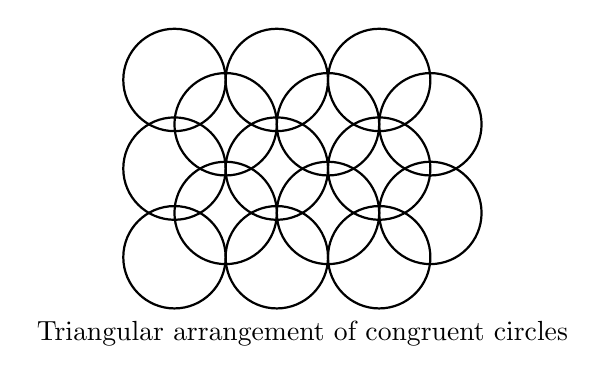
\begin{tikzpicture}[scale=.65]

\foreach \y in {0,1.732,3.464}{
    \foreach \x in {0,2,4}{
        \draw[thick] (\x,\y) circle (1);
    }
}

\foreach \x in {1,3,5}{
    \draw[thick] (\x,.866) circle (1);
    \draw[thick] (\x,2.598) circle (1);
}

\node at (2.5,-1.5) {Triangular arrangement of congruent circles};

\end{tikzpicture}
\end{centereddiagram}

The optimal density of congruent circle packings in the Euclidean plane is

\[
\boxed{
\frac{\pi}{\sqrt{12}}
=
\frac{\pi}{2\sqrt3}
\approx0.9069.
}
\]

%%%%%%%%%%%%%%%%%%%%%%%%%%%%%%%%%%%%%%%%%%%%%%%%%%%%%%%%%%%%
\subsection{Packing Density}
\label{subsec:packing-density}
%%%%%%%%%%%%%%%%%%%%%%%%%%%%%%%%%%%%%%%%%%%%%%%%%%%%%%%%%%%%

Packing density measures the fraction of space occupied by the packed
objects.

For a periodic packing, one may compute

\[
\boxed{
\delta
=
\frac{
\text{volume occupied inside a fundamental region}
}{
\text{volume of the fundamental region}
}.
}
\]

The lowercase Greek letter

\[
\delta
\]

is read ``delta.''

%%%%%%%%%%%%%%%%%%%%%%%%%%%%%%%%%%%%%%%%%%%%%%%%%%%%%%%%%%%%
\subsection{Sphere Packing}
\label{subsec:sphere-packing}
%%%%%%%%%%%%%%%%%%%%%%%%%%%%%%%%%%%%%%%%%%%%%%%%%%%%%%%%%%%%

The three-dimensional sphere-packing problem asks for the densest possible
packing of congruent spheres in \(\R^3\).

The optimal density is

\[
\boxed{
\frac{\pi}{3\sqrt2}
\approx0.74048.
}
\]

This density occurs in the familiar face-centered cubic and hexagonal
close-packed arrangements.

The statement that no denser packing exists is known as the
\emph{Kepler conjecture}, now a theorem.

%%%%%%%%%%%%%%%%%%%%%%%%%%%%%%%%%%%%%%%%%%%%%%%%%%%%%%%%%%%%
\subsection{Higher-Dimensional Sphere Packing}
\label{subsec:higher-dimensional-sphere-packing}
%%%%%%%%%%%%%%%%%%%%%%%%%%%%%%%%%%%%%%%%%%%%%%%%%%%%%%%%%%%%

Sphere packing extends naturally to

\[
\R^n.
\]

The problem becomes increasingly difficult as the dimension grows.

Remarkable exact optimality results are known in certain special dimensions,
including dimensions

\[
8
\]

and

\[
24,
\]

which are associated with the

\[
E_8
\]

lattice and the Leech lattice.

These structures also appear in coding theory, group theory, and mathematical
physics.

%%%%%%%%%%%%%%%%%%%%%%%%%%%%%%%%%%%%%%%%%%%%%%%%%%%%%%%%%%%%
\subsection{Coverings}
\label{subsec:geometric-coverings}
%%%%%%%%%%%%%%%%%%%%%%%%%%%%%%%%%%%%%%%%%%%%%%%%%%%%%%%%%%%%

\begin{definitionbox}{Covering}
A \emph{covering} is an arrangement of sets whose union contains the entire
space or target region.
\end{definitionbox}

Unlike a packing, overlaps are allowed.

Thus packing asks

\[
\boxed{
\text{How densely can objects fit without overlap?}
}
\]

while covering asks

\[
\boxed{
\text{How efficiently can objects cover everything?}
}
\]

%%%%%%%%%%%%%%%%%%%%%%%%%%%%%%%%%%%%%%%%%%%%%%%%%%%%%%%%%%%%
\subsection{Tilings}
\label{subsec:geometric-tilings}
%%%%%%%%%%%%%%%%%%%%%%%%%%%%%%%%%%%%%%%%%%%%%%%%%%%%%%%%%%%%

\begin{definitionbox}{Tiling}
A \emph{tiling}, or \emph{tessellation}, covers a region using tiles whose
interiors do not overlap.
\end{definitionbox}

Thus a tiling simultaneously behaves like a packing and a covering.

Common planar tilings use

\[
\boxed{
\text{triangles},
\quad
\text{squares},
\quad
\text{hexagons}.
}
\]

%%%%%%%%%%%%%%%%%%%%%%%%%%%%%%%%%%%%%%%%%%%%%%%%%%%%%%%%%%%%
\subsection{Regular Euclidean Tilings}
\label{subsec:regular-euclidean-tilings}
%%%%%%%%%%%%%%%%%%%%%%%%%%%%%%%%%%%%%%%%%%%%%%%%%%%%%%%%%%%%

A regular tiling of the Euclidean plane uses one type of regular polygon,
with the same number meeting at every vertex.

There are exactly three regular Euclidean tilings:

\[
\boxed{
\{3,6\},
\qquad
\{4,4\},
\qquad
\{6,3\}.
}
\]

The notation

\[
\{p,q\}
\]

is called a \emph{Schl\"afli symbol}.

It indicates regular \(p\)-gons with \(q\) polygons meeting at each vertex.

%%%%%%%%%%%%%%%%%%%%%%%%%%%%%%%%%%%%%%%%%%%%%%%%%%%%%%%%%%%%
\subsection{Angle Condition for Regular Tilings}
\label{subsec:regular-tiling-angle-condition}
%%%%%%%%%%%%%%%%%%%%%%%%%%%%%%%%%%%%%%%%%%%%%%%%%%%%%%%%%%%%

A regular \(p\)-gon has interior angle

\[
\boxed{
\frac{(p-2)\pi}{p}.
}
\]

For \(q\) copies to meet around a Euclidean vertex,

\[
q\frac{(p-2)\pi}{p}
=
2\pi.
\]

Therefore

\[
\boxed{
\frac1p+\frac1q=\frac12.
}
\]

The positive integer solutions with \(p,q\geq3\) are precisely

\[
\boxed{
(3,6),
\quad
(4,4),
\quad
(6,3).
}
\]

%%%%%%%%%%%%%%%%%%%%%%%%%%%%%%%%%%%%%%%%%%%%%%%%%%%%%%%%%%%%
\subsection{Periodic and Aperiodic Tilings}
\label{subsec:periodic-aperiodic-tilings}
%%%%%%%%%%%%%%%%%%%%%%%%%%%%%%%%%%%%%%%%%%%%%%%%%%%%%%%%%%%%

A tiling is \emph{periodic} if some nonzero translation maps the entire
tiling to itself.

Not every tiling is periodic.

An \emph{aperiodic} tiling has no translational period.

Certain finite collections of tiles can force every valid tiling made from
them to be nonperiodic.

Penrose tilings are famous examples of aperiodic tilings.

%%%%%%%%%%%%%%%%%%%%%%%%%%%%%%%%%%%%%%%%%%%%%%%%%%%%%%%%%%%%
\subsection{Voronoi Diagrams}
\label{subsec:voronoi-diagrams}
%%%%%%%%%%%%%%%%%%%%%%%%%%%%%%%%%%%%%%%%%%%%%%%%%%%%%%%%%%%%

Let

\[
P=\{p_1,\ldots,p_m\}\subseteq\R^n
\]

be a collection of sites.

\begin{definitionbox}{Voronoi Cell}
The \emph{Voronoi cell} of \(p_i\) is

\[
\boxed{
V_i
=
\{
x\in\R^n:
\|x-p_i\|
\leq
\|x-p_j\|
\text{ for every }j
\}.
}
\]
\end{definitionbox}

Thus \(V_i\) consists of all points at least as close to \(p_i\) as to any
other site.

The collection of all cells forms the \emph{Voronoi diagram}.

%%%%%%%%%%%%%%%%%%%%%%%%%%%%%%%%%%%%%%%%%%%%%%%%%%%%%%%%%%%%
\subsection{Geometry of Voronoi Cells}
\label{subsec:voronoi-cell-geometry}
%%%%%%%%%%%%%%%%%%%%%%%%%%%%%%%%%%%%%%%%%%%%%%%%%%%%%%%%%%%%

For two sites \(p_i\) and \(p_j\), the inequality

\[
\|x-p_i\|
\leq
\|x-p_j\|
\]

defines a half-space.

Its boundary is the perpendicular bisector hyperplane of the segment joining
the two sites.

Therefore a Voronoi cell can be written as an intersection of half-spaces.

Hence

\[
\boxed{
\text{every Euclidean Voronoi cell is convex}.
}
\]

%%%%%%%%%%%%%%%%%%%%%%%%%%%%%%%%%%%%%%%%%%%%%%%%%%%%%%%%%%%%
\subsection{Voronoi Diagram Example}
\label{subsec:voronoi-example}
%%%%%%%%%%%%%%%%%%%%%%%%%%%%%%%%%%%%%%%%%%%%%%%%%%%%%%%%%%%%

\begin{centereddiagram}
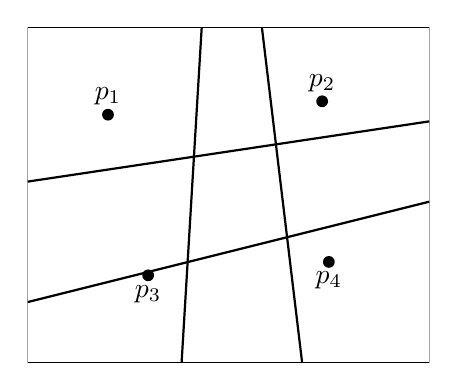
\begin{tikzpicture}[scale=.85]
\clip (-3,-2.5) rectangle (3,2.5);

\draw[thick] (-.7,-2.5)--(-.4,2.5);
\draw[thick] (-3,.2)--(3,1.1);
\draw[thick] (-3,-1.6)--(3,-.1);
\draw[thick] (1.1,-2.5)--(.5,2.5);

\fill (-1.8,1.2) circle (2.5pt) node[above] {$p_1$};
\fill (1.4,1.4) circle (2.5pt) node[above] {$p_2$};
\fill (-1.2,-1.2) circle (2.5pt) node[below] {$p_3$};
\fill (1.5,-1) circle (2.5pt) node[below] {$p_4$};

\draw (-3,-2.5) rectangle (3,2.5);
\end{tikzpicture}
\end{centereddiagram}

The diagram is schematic; exact Voronoi boundaries are determined by
perpendicular bisectors between sites.

%%%%%%%%%%%%%%%%%%%%%%%%%%%%%%%%%%%%%%%%%%%%%%%%%%%%%%%%%%%%
\subsection{Delaunay Triangulations}
\label{subsec:delaunay-triangulations}
%%%%%%%%%%%%%%%%%%%%%%%%%%%%%%%%%%%%%%%%%%%%%%%%%%%%%%%%%%%%

The geometric dual of a Voronoi diagram is the
\emph{Delaunay triangulation}.

Two sites are joined by a Delaunay edge when their Voronoi cells share an
edge in the planar nondegenerate case.

For points in general position, the resulting planar structure is a
triangulation.

%%%%%%%%%%%%%%%%%%%%%%%%%%%%%%%%%%%%%%%%%%%%%%%%%%%%%%%%%%%%
\subsection{Empty Circumcircle Property}
\label{subsec:delaunay-empty-circle}
%%%%%%%%%%%%%%%%%%%%%%%%%%%%%%%%%%%%%%%%%%%%%%%%%%%%%%%%%%%%

A defining property of a planar Delaunay triangulation is the
\emph{empty circumcircle condition}.

For each Delaunay triangle, the interior of its circumcircle contains no
site from the point configuration.

Thus

\[
\boxed{
\text{Delaunay triangle}
\Longrightarrow
\text{empty circumcircle}.
}
\]

If four or more sites are cocircular, the Delaunay triangulation may not be
unique.

%%%%%%%%%%%%%%%%%%%%%%%%%%%%%%%%%%%%%%%%%%%%%%%%%%%%%%%%%%%%
\subsection{Triangulations}
\label{subsec:discrete-triangulations}
%%%%%%%%%%%%%%%%%%%%%%%%%%%%%%%%%%%%%%%%%%%%%%%%%%%%%%%%%%%%

A \emph{triangulation} subdivides a geometric region into simplices.

In the plane, these simplices are triangles.

For a polygon, a triangulation uses noncrossing diagonals to divide the
polygon into triangles.

%%%%%%%%%%%%%%%%%%%%%%%%%%%%%%%%%%%%%%%%%%%%%%%%%%%%%%%%%%%%
\subsection{Triangulating a Convex Polygon}
\label{subsec:triangulating-convex-polygon}
%%%%%%%%%%%%%%%%%%%%%%%%%%%%%%%%%%%%%%%%%%%%%%%%%%%%%%%%%%%%

A convex polygon with \(n\) vertices can be triangulated using

\[
\boxed{
n-3
}
\]

diagonals.

The resulting number of triangles is

\[
\boxed{
n-2.
}
\]

For example, a hexagon can be divided into

\[
6-2=4
\]

triangles.

%%%%%%%%%%%%%%%%%%%%%%%%%%%%%%%%%%%%%%%%%%%%%%%%%%%%%%%%%%%%
\subsection{Counting Polygon Triangulations}
\label{subsec:counting-polygon-triangulations}
%%%%%%%%%%%%%%%%%%%%%%%%%%%%%%%%%%%%%%%%%%%%%%%%%%%%%%%%%%%%

The number of distinct triangulations of a convex \(n\)-gon is

\[
\boxed{
C_{n-2},
}
\]

where

\[
C_k
=
\frac{1}{k+1}\binom{2k}{k}
\]

is the \(k\)-th Catalan number.

Therefore the number of triangulations is

\[
\boxed{
\frac{1}{n-1}
\binom{2n-4}{n-2}.
}
\]

This provides a direct connection between discrete geometry and
combinatorics.

%%%%%%%%%%%%%%%%%%%%%%%%%%%%%%%%%%%%%%%%%%%%%%%%%%%%%%%%%%%%
\subsection{Polytopes}
\label{subsec:discrete-polytopes}
%%%%%%%%%%%%%%%%%%%%%%%%%%%%%%%%%%%%%%%%%%%%%%%%%%%%%%%%%%%%

As introduced in Convex Geometry, a polytope is the convex hull of finitely
many points.

Discrete geometry studies not only the metric shape of a polytope but also
its combinatorial structure.

Important features include:

\[
\boxed{
\text{vertices},
\quad
\text{edges},
\quad
\text{faces},
\quad
\text{facets}.
}
\]

%%%%%%%%%%%%%%%%%%%%%%%%%%%%%%%%%%%%%%%%%%%%%%%%%%%%%%%%%%%%
\subsection{Faces and Facets}
\label{subsec:faces-and-facets}
%%%%%%%%%%%%%%%%%%%%%%%%%%%%%%%%%%%%%%%%%%%%%%%%%%%%%%%%%%%%

A \(k\)-dimensional face is often called a \(k\)-face.

Thus:

\[
\boxed{
0\text{-face}=\text{vertex},
}
\]

\[
\boxed{
1\text{-face}=\text{edge}.
}
\]

For an \(n\)-dimensional polytope, an \((n-1)\)-dimensional face is called a
\emph{facet}.

%%%%%%%%%%%%%%%%%%%%%%%%%%%%%%%%%%%%%%%%%%%%%%%%%%%%%%%%%%%%
\subsection{Euler's Polyhedron Formula}
\label{subsec:euler-polyhedron-formula}
%%%%%%%%%%%%%%%%%%%%%%%%%%%%%%%%%%%%%%%%%%%%%%%%%%%%%%%%%%%%

For a convex three-dimensional polyhedron, let

\[
V=\text{number of vertices},
\]

\[
E=\text{number of edges},
\]

and

\[
F=\text{number of faces}.
\]

Then

\[
\boxed{
V-E+F=2.
}
\]

This is Euler's polyhedron formula.

It is one of the earliest examples of a topological invariant arising from
a geometric object.

%%%%%%%%%%%%%%%%%%%%%%%%%%%%%%%%%%%%%%%%%%%%%%%%%%%%%%%%%%%%
\subsection{Worked Example: Euler's Formula}
\label{subsec:worked-euler-polyhedron}
%%%%%%%%%%%%%%%%%%%%%%%%%%%%%%%%%%%%%%%%%%%%%%%%%%%%%%%%%%%%

\begin{workedexamplebox}{Verify Euler's Formula for a Cube}

A cube has

\[
V=8
\]

vertices,

\[
E=12
\]

edges, and

\[
F=6
\]

faces.

Therefore

\[
V-E+F
=
8-12+6
=
2.
\]

\begin{answerbox}
\[
\boxed{
8-12+6=2
}
\]
\end{answerbox}
\end{workedexamplebox}

%%%%%%%%%%%%%%%%%%%%%%%%%%%%%%%%%%%%%%%%%%%%%%%%%%%%%%%%%%%%
\subsection{The \(f\)-Vector}
\label{subsec:polytope-f-vector}
%%%%%%%%%%%%%%%%%%%%%%%%%%%%%%%%%%%%%%%%%%%%%%%%%%%%%%%%%%%%

The numbers of faces of different dimensions can be recorded in an
\(f\)-vector.

For a \(d\)-dimensional polytope,

\[
\boxed{
(f_0,f_1,\ldots,f_{d-1}),
}
\]

where

\[
f_k
\]

is the number of \(k\)-dimensional faces.

For a cube,

\[
\boxed{
(f_0,f_1,f_2)=(8,12,6).
}
\]

For a tetrahedron,

\[
\boxed{
(f_0,f_1,f_2)=(4,6,4).
}
\]

%%%%%%%%%%%%%%%%%%%%%%%%%%%%%%%%%%%%%%%%%%%%%%%%%%%%%%%%%%%%
\subsection{Regular Polytopes}
\label{subsec:regular-polytopes}
%%%%%%%%%%%%%%%%%%%%%%%%%%%%%%%%%%%%%%%%%%%%%%%%%%%%%%%%%%%%

A regular polytope has maximal symmetry: its faces are congruent regular
polytopes arranged identically around each lower-dimensional face.

In three dimensions, the regular convex polyhedra are the five Platonic
solids:

\[
\boxed{
\text{tetrahedron},
\quad
\text{cube},
\quad
\text{octahedron},
\quad
\text{dodecahedron},
\quad
\text{icosahedron}.
}
\]

%%%%%%%%%%%%%%%%%%%%%%%%%%%%%%%%%%%%%%%%%%%%%%%%%%%%%%%%%%%%
\subsection{Schl\"afli Symbols for Regular Polyhedra}
\label{subsec:schlafli-polyhedra}
%%%%%%%%%%%%%%%%%%%%%%%%%%%%%%%%%%%%%%%%%%%%%%%%%%%%%%%%%%%%

A regular polyhedron has Schl\"afli symbol

\[
\boxed{
\{p,q\},
}
\]

where each face is a regular \(p\)-gon and \(q\) faces meet at every vertex.

For example,

\[
\boxed{
\text{cube}=\{4,3\},
}
\]

while

\[
\boxed{
\text{octahedron}=\{3,4\}.
}
\]

These two polyhedra are dual to each other.

%%%%%%%%%%%%%%%%%%%%%%%%%%%%%%%%%%%%%%%%%%%%%%%%%%%%%%%%%%%%
\subsection{Dual Polytopes}
\label{subsec:dual-polytopes}
%%%%%%%%%%%%%%%%%%%%%%%%%%%%%%%%%%%%%%%%%%%%%%%%%%%%%%%%%%%%

Polytope duality reverses the incidence structure of faces.

Informally,

\[
\boxed{
\text{vertices}
\longleftrightarrow
\text{facets}.
}
\]

For the Platonic solids,

\[
\boxed{
\text{cube}
\longleftrightarrow
\text{octahedron},
}
\]

and

\[
\boxed{
\text{dodecahedron}
\longleftrightarrow
\text{icosahedron}.
}
\]

The tetrahedron is combinatorially self-dual.

%%%%%%%%%%%%%%%%%%%%%%%%%%%%%%%%%%%%%%%%%%%%%%%%%%%%%%%%%%%%
\subsection{Geometric Graphs}
\label{subsec:geometric-graphs}
%%%%%%%%%%%%%%%%%%%%%%%%%%%%%%%%%%%%%%%%%%%%%%%%%%%%%%%%%%%%

A geometric graph consists of vertices represented by points in a geometric
space and edges represented by geometric connections between them.

The geometry of the embedding may impose additional conditions.

Examples include:

\[
\boxed{
\text{planar straight-line graphs},
}
\]

\[
\boxed{
\text{unit-distance graphs},
}
\]

and

\[
\boxed{
\text{proximity graphs}.
}
\]

%%%%%%%%%%%%%%%%%%%%%%%%%%%%%%%%%%%%%%%%%%%%%%%%%%%%%%%%%%%%
\subsection{Unit-Distance Graphs}
\label{subsec:unit-distance-graphs}
%%%%%%%%%%%%%%%%%%%%%%%%%%%%%%%%%%%%%%%%%%%%%%%%%%%%%%%%%%%%

A unit-distance graph is a graph whose vertices can be represented by points
in the plane so that every graph edge has length \(1\).

Not every pair of points at distance \(1\) must necessarily be connected
unless one specifically requires a faithful unit-distance representation.

Such graphs connect graph theory with Euclidean geometry.

%%%%%%%%%%%%%%%%%%%%%%%%%%%%%%%%%%%%%%%%%%%%%%%%%%%%%%%%%%%%
\subsection{Nearest-Neighbor Graphs}
\label{subsec:nearest-neighbor-graphs}
%%%%%%%%%%%%%%%%%%%%%%%%%%%%%%%%%%%%%%%%%%%%%%%%%%%%%%%%%%%%

Given a point configuration, one may connect each point to one or more of
its nearest neighbors.

This produces a geometric graph reflecting local spatial relationships.

Nearest-neighbor structures appear in

\[
\boxed{
\text{data analysis},
\quad
\text{pattern recognition},
\quad
\text{spatial statistics},
\quad
\text{machine learning}.
}
\]

%%%%%%%%%%%%%%%%%%%%%%%%%%%%%%%%%%%%%%%%%%%%%%%%%%%%%%%%%%%%
\subsection{Euclidean Minimum Spanning Trees}
\label{subsec:euclidean-mst}
%%%%%%%%%%%%%%%%%%%%%%%%%%%%%%%%%%%%%%%%%%%%%%%%%%%%%%%%%%%%

Given points

\[
p_1,\ldots,p_n,
\]

form the complete weighted graph in which the edge between \(p_i\) and
\(p_j\) has weight

\[
\|p_i-p_j\|.
\]

A \emph{Euclidean minimum spanning tree} is a spanning tree of minimum total
edge length.

It connects all points while minimizing

\[
\boxed{
\sum_{\text{tree edges }ij}
\|p_i-p_j\|.
}
\]

%%%%%%%%%%%%%%%%%%%%%%%%%%%%%%%%%%%%%%%%%%%%%%%%%%%%%%%%%%%%
\subsection{Incidence Geometry}
\label{subsec:discrete-incidence-geometry}
%%%%%%%%%%%%%%%%%%%%%%%%%%%%%%%%%%%%%%%%%%%%%%%%%%%%%%%%%%%%

An \emph{incidence} records when geometric objects meet.

For example, a point-line incidence occurs when a point lies on a line.

Given a finite set of points \(P\) and lines \(L\), one may ask for the
number

\[
\boxed{
I(P,L)
=
|\{(p,\ell)\in P\times L:p\in\ell\}|.
}
\]

Bounding incidence counts is a major topic in discrete geometry.

%%%%%%%%%%%%%%%%%%%%%%%%%%%%%%%%%%%%%%%%%%%%%%%%%%%%%%%%%%%%
\subsection{The Szemer\'edi--Trotter Theorem}
\label{subsec:szemeredi-trotter}
%%%%%%%%%%%%%%%%%%%%%%%%%%%%%%%%%%%%%%%%%%%%%%%%%%%%%%%%%%%%

A central incidence theorem concerns points and lines in the plane.

\begin{theorem}[Szemer\'edi--Trotter Theorem]
For a finite set \(P\) of points and a finite set \(L\) of lines in
\(\R^2\),

\[
\boxed{
I(P,L)
=
O\left(
|P|^{2/3}|L|^{2/3}
+
|P|
+
|L|
\right).
}
\]
\end{theorem}

The notation

\[
O(\cdot)
\]

is read ``big O'' and denotes an asymptotic upper bound up to a constant
factor.

This theorem is a cornerstone of combinatorial incidence geometry.

%%%%%%%%%%%%%%%%%%%%%%%%%%%%%%%%%%%%%%%%%%%%%%%%%%%%%%%%%%%%
\subsection{Distinct Distance Problems}
\label{subsec:distinct-distance-problems}
%%%%%%%%%%%%%%%%%%%%%%%%%%%%%%%%%%%%%%%%%%%%%%%%%%%%%%%%%%%%

Given \(n\) points in the plane, how few distinct pairwise distances can
they determine?

This is the classical Erd\H{o}s distinct distances problem.

The question illustrates the typical style of discrete geometry:

\[
\boxed{
\text{finite configuration}
+
\text{geometric constraint}
+
\text{extremal counting}.
}
\]

%%%%%%%%%%%%%%%%%%%%%%%%%%%%%%%%%%%%%%%%%%%%%%%%%%%%%%%%%%%%
\subsection{The Kissing Number Problem}
\label{subsec:kissing-number}
%%%%%%%%%%%%%%%%%%%%%%%%%%%%%%%%%%%%%%%%%%%%%%%%%%%%%%%%%%%%

The \emph{kissing number} in dimension \(n\) is the maximum number of
nonoverlapping unit spheres that can simultaneously touch another unit
sphere.

In two dimensions,

\[
\boxed{
\tau_2=6.
}
\]

In three dimensions,

\[
\boxed{
\tau_3=12.
}
\]

The symbol

\[
\tau
\]

is the lowercase Greek letter ``tau.''

%%%%%%%%%%%%%%%%%%%%%%%%%%%%%%%%%%%%%%%%%%%%%%%%%%%%%%%%%%%%
\subsection{Discrete Isoperimetric Questions}
\label{subsec:discrete-isoperimetric}
%%%%%%%%%%%%%%%%%%%%%%%%%%%%%%%%%%%%%%%%%%%%%%%%%%%%%%%%%%%%

Classical isoperimetric problems compare boundary size with enclosed volume.

Discrete analogues ask similar questions for graphs, lattices, polytopes,
and finite subsets.

A typical question is:

\begin{quote}
Among all finite sets of a given size, which arrangement minimizes the size
of its boundary?
\end{quote}

These problems connect discrete geometry with combinatorics and optimization.

%%%%%%%%%%%%%%%%%%%%%%%%%%%%%%%%%%%%%%%%%%%%%%%%%%%%%%%%%%%%
\subsection{Discrete Geometry and Coding Theory}
\label{subsec:discrete-geometry-coding}
%%%%%%%%%%%%%%%%%%%%%%%%%%%%%%%%%%%%%%%%%%%%%%%%%%%%%%%%%%%%

Error-correcting codes can be interpreted geometrically.

Codewords are points in a metric space, and reliable decoding requires them
to be sufficiently separated.

Thus coding problems resemble sphere-packing problems:

\[
\boxed{
\text{maximize the number of points}
}
\]

subject to

\[
\boxed{
\text{a minimum-distance constraint}.
}
\]

This geometric interpretation is particularly important for lattice codes
and spherical codes.

%%%%%%%%%%%%%%%%%%%%%%%%%%%%%%%%%%%%%%%%%%%%%%%%%%%%%%%%%%%%
\subsection{Spherical Codes}
\label{subsec:spherical-codes}
%%%%%%%%%%%%%%%%%%%%%%%%%%%%%%%%%%%%%%%%%%%%%%%%%%%%%%%%%%%%

A spherical code is a finite collection of points on a sphere with prescribed
angular separation.

One seeks configurations maximizing the minimum angle between points or
maximizing the number of points subject to a minimum-angle requirement.

Spherical codes connect

\[
\boxed{
\text{discrete geometry},
\quad
\text{information theory},
\quad
\text{optimization}.
}
\]

%%%%%%%%%%%%%%%%%%%%%%%%%%%%%%%%%%%%%%%%%%%%%%%%%%%%%%%%%%%%
\subsection{Discrete Geometry and Crystallography}
\label{subsec:discrete-geometry-crystallography}
%%%%%%%%%%%%%%%%%%%%%%%%%%%%%%%%%%%%%%%%%%%%%%%%%%%%%%%%%%%%

Crystalline materials exhibit repeating spatial structures.

Lattices provide mathematical models for these periodic arrangements.

A crystal structure can often be described using

\[
\boxed{
\text{a lattice}
+
\text{a finite motif}.
}
\]

Translations of the motif by lattice vectors generate the repeating
structure.

%%%%%%%%%%%%%%%%%%%%%%%%%%%%%%%%%%%%%%%%%%%%%%%%%%%%%%%%%%%%
\subsection{Discrete Geometry and Optimization}
\label{subsec:discrete-geometry-optimization}
%%%%%%%%%%%%%%%%%%%%%%%%%%%%%%%%%%%%%%%%%%%%%%%%%%%%%%%%%%%%

Many optimization problems contain geometric and discrete components.

Examples include:

\[
\boxed{
\text{facility location},
}
\]

\[
\boxed{
\text{packing and covering},
}
\]

\[
\boxed{
\text{network design},
}
\]

\[
\boxed{
\text{mesh generation},
}
\]

and

\[
\boxed{
\text{integer programming}.
}
\]

The combination of convex geometry and discrete structure is especially
important in mixed-integer optimization.

%%%%%%%%%%%%%%%%%%%%%%%%%%%%%%%%%%%%%%%%%%%%%%%%%%%%%%%%%%%%
\subsection{Common Errors}
\label{subsec:discrete-geometry-common-errors}
%%%%%%%%%%%%%%%%%%%%%%%%%%%%%%%%%%%%%%%%%%%%%%%%%%%%%%%%%%%%

\subsubsection{Assuming Discrete Means Finite}

A discrete set need not be finite.

For example,

\[
\boxed{
\Z^n
}
\]

is infinite but discrete.

%%%%%%%%%%%%%%%%%%%%%%%%%%%%%%%%%%%%%%%%%%%%%%%%%%%%%%%%%%%%
\subsubsection{Confusing a Lattice with an Arbitrary Point Set}

A lattice has algebraic structure.

Its points are integer combinations of basis vectors.

An arbitrary discrete point configuration need not form a lattice.

%%%%%%%%%%%%%%%%%%%%%%%%%%%%%%%%%%%%%%%%%%%%%%%%%%%%%%%%%%%%
\subsubsection{Confusing a Lattice Basis with a Vector-Space Basis}

A lattice basis generates lattice points using

\[
\boxed{
\text{integer coefficients}.
}
\]

A vector-space basis generates all vectors using real coefficients.

The same vectors may serve both roles, but the allowed coefficients differ.

%%%%%%%%%%%%%%%%%%%%%%%%%%%%%%%%%%%%%%%%%%%%%%%%%%%%%%%%%%%%
\subsubsection{Forgetting the Absolute Value in the Lattice Determinant}

The covolume is

\[
\boxed{
|\det B|,
}
\]

not necessarily \(\det B\).

Volume must be nonnegative.

%%%%%%%%%%%%%%%%%%%%%%%%%%%%%%%%%%%%%%%%%%%%%%%%%%%%%%%%%%%%
\subsubsection{Using Pick's Theorem for Arbitrary Polygons}

Pick's theorem applies to simple lattice polygons.

The vertices must lie on lattice points, and self-intersecting polygons
require additional care and different formulations.

%%%%%%%%%%%%%%%%%%%%%%%%%%%%%%%%%%%%%%%%%%%%%%%%%%%%%%%%%%%%
\subsubsection{Confusing Interior and Boundary Counts}

In Pick's theorem,

\[
I
\]

counts lattice points strictly inside the polygon.

The quantity

\[
B
\]

counts lattice points on the boundary.

Do not count a boundary point as an interior point.

%%%%%%%%%%%%%%%%%%%%%%%%%%%%%%%%%%%%%%%%%%%%%%%%%%%%%%%%%%%%
\subsubsection{Confusing Packing with Covering}

A packing forbids interior overlap.

A covering requires the target region to be completely covered.

A tiling does both.

%%%%%%%%%%%%%%%%%%%%%%%%%%%%%%%%%%%%%%%%%%%%%%%%%%%%%%%%%%%%
\subsubsection{Assuming the Square Circle Packing Is Optimal}

The square lattice produces a simple circle packing, but it is not the
densest planar packing.

The triangular arrangement is denser.

%%%%%%%%%%%%%%%%%%%%%%%%%%%%%%%%%%%%%%%%%%%%%%%%%%%%%%%%%%%%
\subsubsection{Treating Voronoi Boundaries as Arbitrary}

Voronoi boundaries arise from equal-distance conditions.

For two Euclidean sites, the relevant boundary is their perpendicular
bisector hyperplane.

%%%%%%%%%%%%%%%%%%%%%%%%%%%%%%%%%%%%%%%%%%%%%%%%%%%%%%%%%%%%
\subsubsection{Assuming Delaunay Triangulations Are Always Unique}

If four planar sites are cocircular, multiple Delaunay triangulations may
exist.

General-position assumptions remove this ambiguity.

%%%%%%%%%%%%%%%%%%%%%%%%%%%%%%%%%%%%%%%%%%%%%%%%%%%%%%%%%%%%
\subsubsection{Confusing Geometric and Abstract Graphs}

An abstract graph records vertices and adjacency.

A geometric graph additionally represents vertices and edges using geometric
objects, so lengths, crossings, angles, and positions may matter.

%%%%%%%%%%%%%%%%%%%%%%%%%%%%%%%%%%%%%%%%%%%%%%%%%%%%%%%%%%%%
\subsubsection{Applying Euler's Formula to Every Geometric Object}

The formula

\[
V-E+F=2
\]

applies to convex polyhedra and, more generally, appropriate cell
decompositions of the sphere.

Different surfaces have different Euler characteristics.

%%%%%%%%%%%%%%%%%%%%%%%%%%%%%%%%%%%%%%%%%%%%%%%%%%%%%%%%%%%%
\subsection{Applications and Connections}
\label{subsec:discrete-geometry-applications}
%%%%%%%%%%%%%%%%%%%%%%%%%%%%%%%%%%%%%%%%%%%%%%%%%%%%%%%%%%%%

\begin{applicationbox}
\textbf{Number Theory.}
Lattices and convex bodies form the geometry of numbers, where geometric
arguments produce arithmetic conclusions.

\medskip

\textbf{Combinatorics.}
Counting triangulations, incidences, distances, faces, and configurations
connects geometry directly with enumerative and extremal combinatorics.

\medskip

\textbf{Optimization.}
Lattice points, polytopes, packings, coverings, and integer constraints are
central to discrete and mixed-integer optimization.

\medskip

\textbf{Computational Geometry.}
Voronoi diagrams, Delaunay triangulations, convex hulls, geometric graphs,
and spatial search structures are fundamental computational objects.

\medskip

\textbf{Coding Theory.}
Sphere packings, spherical codes, and lattice codes model the separation of
codewords needed for reliable communication.

\medskip

\textbf{Crystallography.}
Lattices and periodic tilings model repeating structures in crystals and
materials.

\medskip

\textbf{Computer Graphics.}
Triangulations and geometric meshes are used to represent surfaces and
three-dimensional objects.

\medskip

\textbf{Geographic Information Systems.}
Voronoi regions can model service areas, nearest facilities, and spatial
influence.

\medskip

\textbf{Data Science.}
Nearest-neighbor graphs, proximity structures, and geometric partitions help
organize high-dimensional data.

\medskip

\textbf{Topology.}
Euler's polyhedron formula foreshadows the Euler characteristic and the
topological study of cell complexes.
\end{applicationbox}

%%%%%%%%%%%%%%%%%%%%%%%%%%%%%%%%%%%%%%%%%%%%%%%%%%%%%%%%%%%%
\subsection{Exercises}
\label{subsec:discrete-geometry-exercises}
%%%%%%%%%%%%%%%%%%%%%%%%%%%%%%%%%%%%%%%%%%%%%%%%%%%%%%%%%%%%

\begin{exercise}[1]
Give an example of an infinite discrete subset of \(\R\).
\end{exercise}

\begin{exercise}[1]
Is

\[
\Z^2
\]

finite? Is it discrete?
\end{exercise}

\begin{exercise}[1]
State the definition of a lattice in \(\R^n\).
\end{exercise}

\begin{exercise}[1]
Find the lattice generated by

\[
v_1=(2,0),
\qquad
v_2=(0,2).
\]
\end{exercise}

\begin{exercise}[1]
Compute the determinant of the lattice generated by

\[
v_1=(3,0),
\qquad
v_2=(0,4).
\]
\end{exercise}

\begin{exercise}[1]
What geometric quantity does the lattice determinant measure?
\end{exercise}

\begin{exercise}[1]
State Pick's theorem.
\end{exercise}

\begin{exercise}[1]
A lattice polygon has

\[
I=4,
\qquad
B=8.
\]

Find its area.
\end{exercise}

\begin{exercise}[1]
A lattice polygon has area \(10\) and \(B=6\). Find \(I\).
\end{exercise}

\begin{exercise}[1]
How many lattice points lie on the segment joining

\[
(0,0)
\]

and

\[
(6,9)?
\]
\end{exercise}

\begin{exercise}[1]
Explain the difference between a packing and a covering.
\end{exercise}

\begin{exercise}[1]
What additional property makes an arrangement a tiling?
\end{exercise}

\begin{exercise}[1]
List the three regular Euclidean tilings.
\end{exercise}

\begin{exercise}[1]
Interpret the Schl\"afli symbol

\[
\{4,4\}.
\]
\end{exercise}

\begin{exercise}[1]
Define a Voronoi cell.
\end{exercise}

\begin{exercise}[1]
What geometric object forms the boundary between the Voronoi regions of two
sites?
\end{exercise}

\begin{exercise}[1]
State the empty circumcircle property of a Delaunay triangulation.
\end{exercise}

\begin{exercise}[1]
How many triangles occur in a triangulation of a convex \(10\)-gon?
\end{exercise}

\begin{exercise}[1]
How many diagonals are used in such a triangulation?
\end{exercise}

\begin{exercise}[1]
State Euler's polyhedron formula.
\end{exercise}

\begin{exercise}[1]
Verify Euler's formula for a tetrahedron.
\end{exercise}

\begin{exercise}[1]
Write the \(f\)-vector of a cube.
\end{exercise}

\begin{exercise}[1]
Write the \(f\)-vector of a tetrahedron.
\end{exercise}

\begin{exercise}[2]
Describe a fundamental parallelogram for the lattice generated by

\[
(2,0)
\]

and

\[
(1,3).
\]
\end{exercise}

\begin{exercise}[2]
Compute the determinant of that lattice.
\end{exercise}

\begin{exercise}[2]
Find the number of lattice points on the segment from

\[
(2,3)
\]

to

\[
(14,11).
\]
\end{exercise}

\begin{exercise}[2]
Use Pick's theorem to find the area of a lattice polygon with

\[
I=11,
\qquad
B=12.
\]
\end{exercise}

\begin{exercise}[2]
A lattice rectangle has vertices

\[
(0,0),\quad(5,0),\quad(5,3),\quad(0,3).
\]

Determine \(I\), \(B\), and verify Pick's theorem.
\end{exercise}

\begin{exercise}[2]
Explain why translations of a fundamental parallelepiped by lattice vectors
tile the ambient space.
\end{exercise}

\begin{exercise}[2]
State the hypotheses of Minkowski's convex body theorem.
\end{exercise}

\begin{exercise}[2]
For \(\Lambda=\Z^2\), what area threshold appears in Minkowski's convex body
theorem?
\end{exercise}

\begin{exercise}[2]
Compute the packing density of congruent circles arranged in a square
lattice with neighboring circles tangent.
\end{exercise}

\begin{exercise}[2]
Compare the square-lattice packing density with

\[
\frac{\pi}{2\sqrt3}.
\]
\end{exercise}

\begin{exercise}[2]
Derive the equation

\[
\frac1p+\frac1q=\frac12
\]

for regular Euclidean tilings.
\end{exercise}

\begin{exercise}[2]
Solve

\[
\frac1p+\frac1q=\frac12
\]

for integers \(p,q\geq3\).
\end{exercise}

\begin{exercise}[2]
Explain why a Euclidean Voronoi cell is convex.
\end{exercise}

\begin{exercise}[2]
For two sites

\[
p_1=(0,0),
\qquad
p_2=(4,0),
\]

find their equal-distance boundary.
\end{exercise}

\begin{exercise}[2]
How many triangulations does a convex pentagon have?
\end{exercise}

\begin{exercise}[2]
How many triangulations does a convex hexagon have?
\end{exercise}

\begin{exercise}[2]
Identify the dual Platonic solid of a cube.
\end{exercise}

\begin{exercise}[2]
Identify the dual Platonic solid of a dodecahedron.
\end{exercise}

\begin{exercise}[2]
Explain why the tetrahedron is combinatorially self-dual.
\end{exercise}

\begin{exercise}[2]
What is the kissing number in dimension \(2\)?
\end{exercise}

\begin{exercise}[2]
What is the kissing number in dimension \(3\)?
\end{exercise}

\begin{exercise}[3]
Prove the formula

\[
\gcd(\Delta x,\Delta y)+1
\]

for the number of lattice points on a lattice segment.
\end{exercise}

\begin{exercise}[3]
Use Pick's theorem to derive the area formula for a lattice triangle in a
simple example.
\end{exercise}

\begin{exercise}[3]
Show that the Voronoi cell of a site is an intersection of half-spaces.
\end{exercise}

\begin{exercise}[3]
Explain the dual relationship between Voronoi diagrams and Delaunay
triangulations.
\end{exercise}

\begin{exercise}[3]
Prove that every triangulation of a convex \(n\)-gon contains exactly

\[
n-2
\]

triangles.
\end{exercise}

\begin{exercise}[3]
Use Euler's formula to derive the relationship between vertices, edges, and
triangular faces of a convex triangulated polyhedron.
\end{exercise}

\begin{exercise}[3]
Show that every tree embedded with straight-line edges and no crossings is a
planar geometric graph.
\end{exercise}

\begin{exercise}[3]
Explain why a Euclidean minimum spanning tree cannot contain a cycle.
\end{exercise}

\begin{exercise}[3]
Explain how sphere packing can model error-correcting codes.
\end{exercise}

\begin{exercise}[3]
Explain how a lattice can model a periodic crystal structure.
\end{exercise}

\begin{exercise}[3]
Describe the difference between an abstract graph and a geometric graph.
\end{exercise}

\begin{exercise}[3]
Explain why Euler's formula is fundamentally topological rather than purely
metric.
\end{exercise}

\begin{exercise}[4]
Research one proof strategy for Pick's theorem.
\end{exercise}

\begin{exercise}[4]
Investigate one number-theoretic application of Minkowski's convex body
theorem.
\end{exercise}

\begin{exercise}[4]
Derive the density

\[
\frac{\pi}{2\sqrt3}
\]

of the triangular circle packing.
\end{exercise}

\begin{exercise}[4]
Research the history and proof of the Kepler conjecture.
\end{exercise}

\begin{exercise}[4]
Investigate why dimensions \(8\) and \(24\) are exceptional in sphere
packing.
\end{exercise}

\begin{exercise}[4]
Research Penrose tilings and explain why they are aperiodic.
\end{exercise}

\begin{exercise}[4]
Investigate the Catalan-number formula for triangulations of a convex
polygon.
\end{exercise}

\begin{exercise}[4]
Research the Szemer\'edi--Trotter theorem and describe one application.
\end{exercise}

\begin{exercise}[4]
Investigate the Erd\H{o}s distinct distances problem.
\end{exercise}

\begin{exercise}[4]
Research spherical codes and explain their connection to communication
theory.
\end{exercise}

%%%%%%%%%%%%%%%%%%%%%%%%%%%%%%%%%%%%%%%%%%%%%%%%%%%%%%%%%%%%
\subsection{Conceptual Summary}
\label{subsec:discrete-geometry-summary}
%%%%%%%%%%%%%%%%%%%%%%%%%%%%%%%%%%%%%%%%%%%%%%%%%%%%%%%%%%%%

Discrete geometry studies finite and countable geometric configurations.

Important examples include

\[
\boxed{
\text{point sets},
\quad
\text{lattices},
\quad
\text{polytopes},
\quad
\text{packings},
\quad
\text{tilings}.
}
\]

A full-rank lattice has the form

\[
\boxed{
\Lambda
=
\left\{
m_1v_1+\cdots+m_nv_n:
m_i\in\Z
\right\}.
}
\]

Its fundamental volume is

\[
\boxed{
\det(\Lambda)=|\det B|.
}
\]

For a simple lattice polygon, Pick's theorem gives

\[
\boxed{
A=I+\frac{B}{2}-1.
}
\]

Minkowski's convex body theorem connects the volume of a centrally symmetric
convex body with the existence of nonzero lattice points.

Packings seek dense nonoverlapping arrangements.

Coverings seek efficient complete coverage.

Tilings cover without overlapping interiors.

Voronoi diagrams partition space according to nearest sites:

\[
\boxed{
V_i
=
\{
x:\|x-p_i\|\leq\|x-p_j\|
\text{ for all }j
\}.
}
\]

Delaunay triangulations provide a dual geometric structure.

A convex \(n\)-gon triangulates into

\[
\boxed{
n-2
}
\]

triangles using

\[
\boxed{
n-3
}
\]

diagonals.

For convex polyhedra,

\[
\boxed{
V-E+F=2.
}
\]

Discrete geometry also studies incidence counts, distinct distances,
geometric graphs, spherical codes, and extremal arrangements.

The subject therefore combines

\[
\boxed{
\text{geometry}
+
\text{combinatorics}
+
\text{number theory}
+
\text{optimization}
+
\text{computation}.
}
\]

%%%%%%%%%%%%%%%%%%%%%%%%%%%%%%%%%%%%%%%%%%%%%%%%%%%%%%%%%%%%
\subsection{Section Connections}
\label{subsec:discrete-geometry-connections}
%%%%%%%%%%%%%%%%%%%%%%%%%%%%%%%%%%%%%%%%%%%%%%%%%%%%%%%%%%%%

\chapterconnection{
Discrete Geometry builds directly on Convex Geometry through convex hulls,
polytopes, supporting structures, and Minkowski's theorem. Lattices connect
the subject with Number Theory and the Geometry of Numbers. Polytope face
counts, polygon triangulations, incidence problems, and geometric graphs
lead into Combinatorics and Graph Theory. Euler's polyhedron formula
foreshadows Euler characteristic and cell complexes in Topology. Packings
and spherical codes connect geometry with Coding Theory and Optimization.
Voronoi diagrams, Delaunay triangulations, geometric graphs, and algorithmic
point-set problems provide the direct foundation for the next section,
Computational Geometry.
}

%%%%%%%%%%%%%%%%%%%%%%%%%%%%%%%%%%%%%%%%%%%%%%%%%%%%%%%%%%%%
% SECTION SOURCE TRACKING
%%%%%%%%%%%%%%%%%%%%%%%%%%%%%%%%%%%%%%%%%%%%%%%%%%%%%%%%%%%%

%------------------------------------------------------------
% 3.12 Discrete Geometry
%------------------------------------------------------------
%
% Source basis:
%   - Standard discrete geometry, geometry of numbers,
%     polyhedral geometry, and combinatorial geometry.
%
% Used for:
%   - discrete point sets;
%   - finite point configurations;
%   - general position;
%   - lattices and lattice bases;
%   - fundamental parallelepipeds;
%   - lattice determinants;
%   - lattice polygons;
%   - Pick's theorem;
%   - lattice points on segments;
%   - geometry of numbers;
%   - Minkowski's convex body theorem;
%   - packings and coverings;
%   - circle and sphere packing;
%   - tilings and tessellations;
%   - regular Euclidean tilings;
%   - periodic and aperiodic tilings;
%   - Voronoi diagrams;
%   - Delaunay triangulations;
%   - polygon triangulations;
%   - Catalan-number connections;
%   - convex polytopes;
%   - Euler's polyhedron formula;
%   - f-vectors;
%   - regular and dual polytopes;
%   - geometric graphs;
%   - Euclidean minimum spanning trees;
%   - incidence geometry;
%   - Szemeredi--Trotter theorem;
%   - distinct-distance problems;
%   - kissing numbers;
%   - spherical codes;
%   - applications to coding and crystallography.
%
% Notes:
%   - Convex hulls, convex bodies, and polyhedral
%     representations are developed canonically in
%     Convex Geometry.
%   - Arithmetic properties of lattices are connected to
%     Number Theory.
%   - Graph-theoretic concepts and Catalan numbers are
%     developed canonically in Discrete Mathematics.
%   - Euler characteristic is developed canonically in
%     Topology.
%   - Voronoi, Delaunay, convex-hull, proximity, and
%     geometric graph algorithms are developed further in
%     Computational Geometry.
%   - The next section completes the Geometry chapter with
%     Computational Geometry.
%
%%%%%%%%%%%%%%%%%%%%%%%%%%%%%%%%%%%%%%%%%%%%%%%%%%%%%%%%%%%%